\chapter{Global Surrogate-Driven Analysis}
\label{ch:global_surrogate}

Chapter~7 established that AUROC saturates at model size \texttt{d64\_L6}
($\sim$202k parameters, $\sim$10.3M FLOPs per event), and that no larger
configuration improves discrimination on the primary 4t-versus-background task.
This chapter takes that model size as fixed and asks a different question: given
the full space of architectural choices explored across Chapters~4--6, which
combination of axes maximises discrimination performance?

The preceding chapters studied architectural axes one family at a time.
Each experiment held most axes fixed and varied a small subset, which
enables controlled causal inference but covers only a fraction of the
joint configuration space. This chapter takes the complementary view:
the full corpus of approximately 983 transformer runs on the primary task
(4t vs.\ combined background, G3 = \texttt{ttH+ttW+ttWW+ttZ | 4t}) is
treated as a large observational dataset, and statistical methods are used
to extract global structure from it.

The chapter proceeds in five stages. Section~\ref{sec:ch8_audit} audits
the run database, defines the primary analysis cohort, and characterises
axis coverage. Section~\ref{sec:ch8_marginals} performs a marginal
sensitivity analysis: for each axis, the range of per-level mean AUROC
is computed and compared to the seed noise floor. Section~\ref{sec:ch8_surrogate}
fits a global XGBoost surrogate on the full axis vector and uses SHAP to
attribute importance to axis families. Section~\ref{sec:ch8_candidates}
proposes and validates new candidate configurations derived from both the
surrogate and a marginal-greedy heuristic, and compares all three search
strategies including an Optuna TPE search. Section~\ref{sec:ch8_summary}
summarises the findings and promotes the best validated candidate to
Chapter~\ref{ch:best_model}.

% ─────────────────────────────────────────────────────────────────────────────
\section{Database Audit and Inclusion Rules}
\label{sec:ch8_audit}

\subsection{Run counts and cohort definition}

The raw W\&B export contains 1\,320 rows across all classification tasks
and spec versions. The primary analysis cohort is formed by applying three
sequential filters. First, only runs on the G3 task (4t vs.\ combined
background) are retained. Second, only runs evaluated under the
\texttt{eval\_v2.1} spec version are included; three legacy runs on an
earlier hash are discarded. Third, runs with missing or failed evaluations
(null \texttt{eval\_v2/test\_auroc}) are removed. The resulting primary
cohort contains \textbf{983 runs}.

Figure~\ref{fig:ch8_audit_spec} shows the distribution of runs by spec
version, confirming that the overwhelming majority (1\,012 of the 1\,015
G3 runs passing all other filters) use \texttt{eval\_v2.1}. The three
legacy runs are excluded from all subsequent analysis.

\begin{figure}[h]
  \centering
  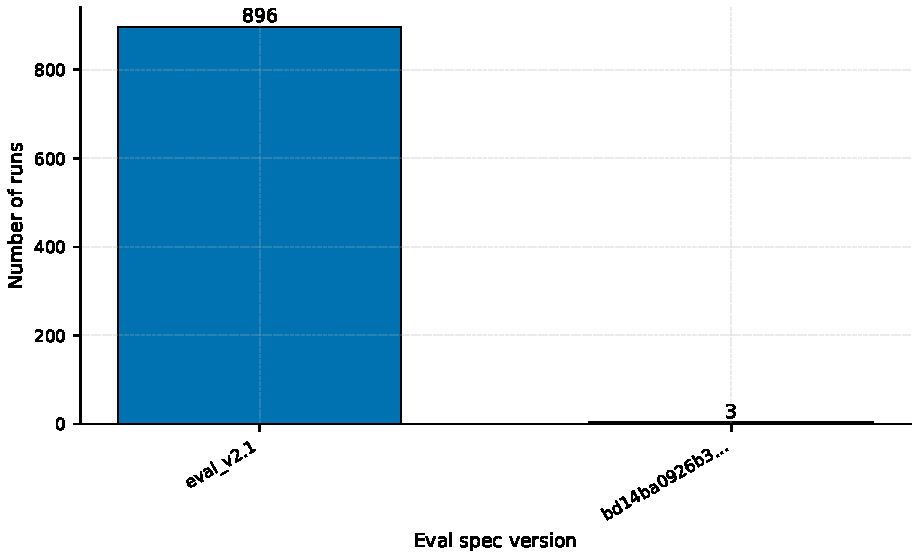
\includegraphics[width=0.75\linewidth]{figures/ch8/audit_run_counts_by_spec.pdf}
  \caption{Run counts by evaluation spec version for the G3 cohort. The
    three runs on the legacy spec version are discarded; all analysis
    uses the 1\,012 runs on \texttt{eval\_v2.1}.}
  \label{fig:ch8_audit_spec}
\end{figure}

\subsection{Axis coverage and co-occurrence structure}

Many axis columns contain missing values by construction: conditional
sub-axes (for example the bias sub-axes \wandbaxis{B1-G2} and \wandbaxis{B1-G3})
are only meaningful when their parent axis is active, and are encoded as
\texttt{NaN} otherwise. Figure~\ref{fig:ch8_missingness} shows the
fraction of missing values per axis column across all three G3 cohorts in
the raw 04 export. High missingness in the B1 sub-axis columns and in the
KAN-specific axes (K3--K5) is structural, not a data quality issue.

\begin{figure}[h]
  \centering
  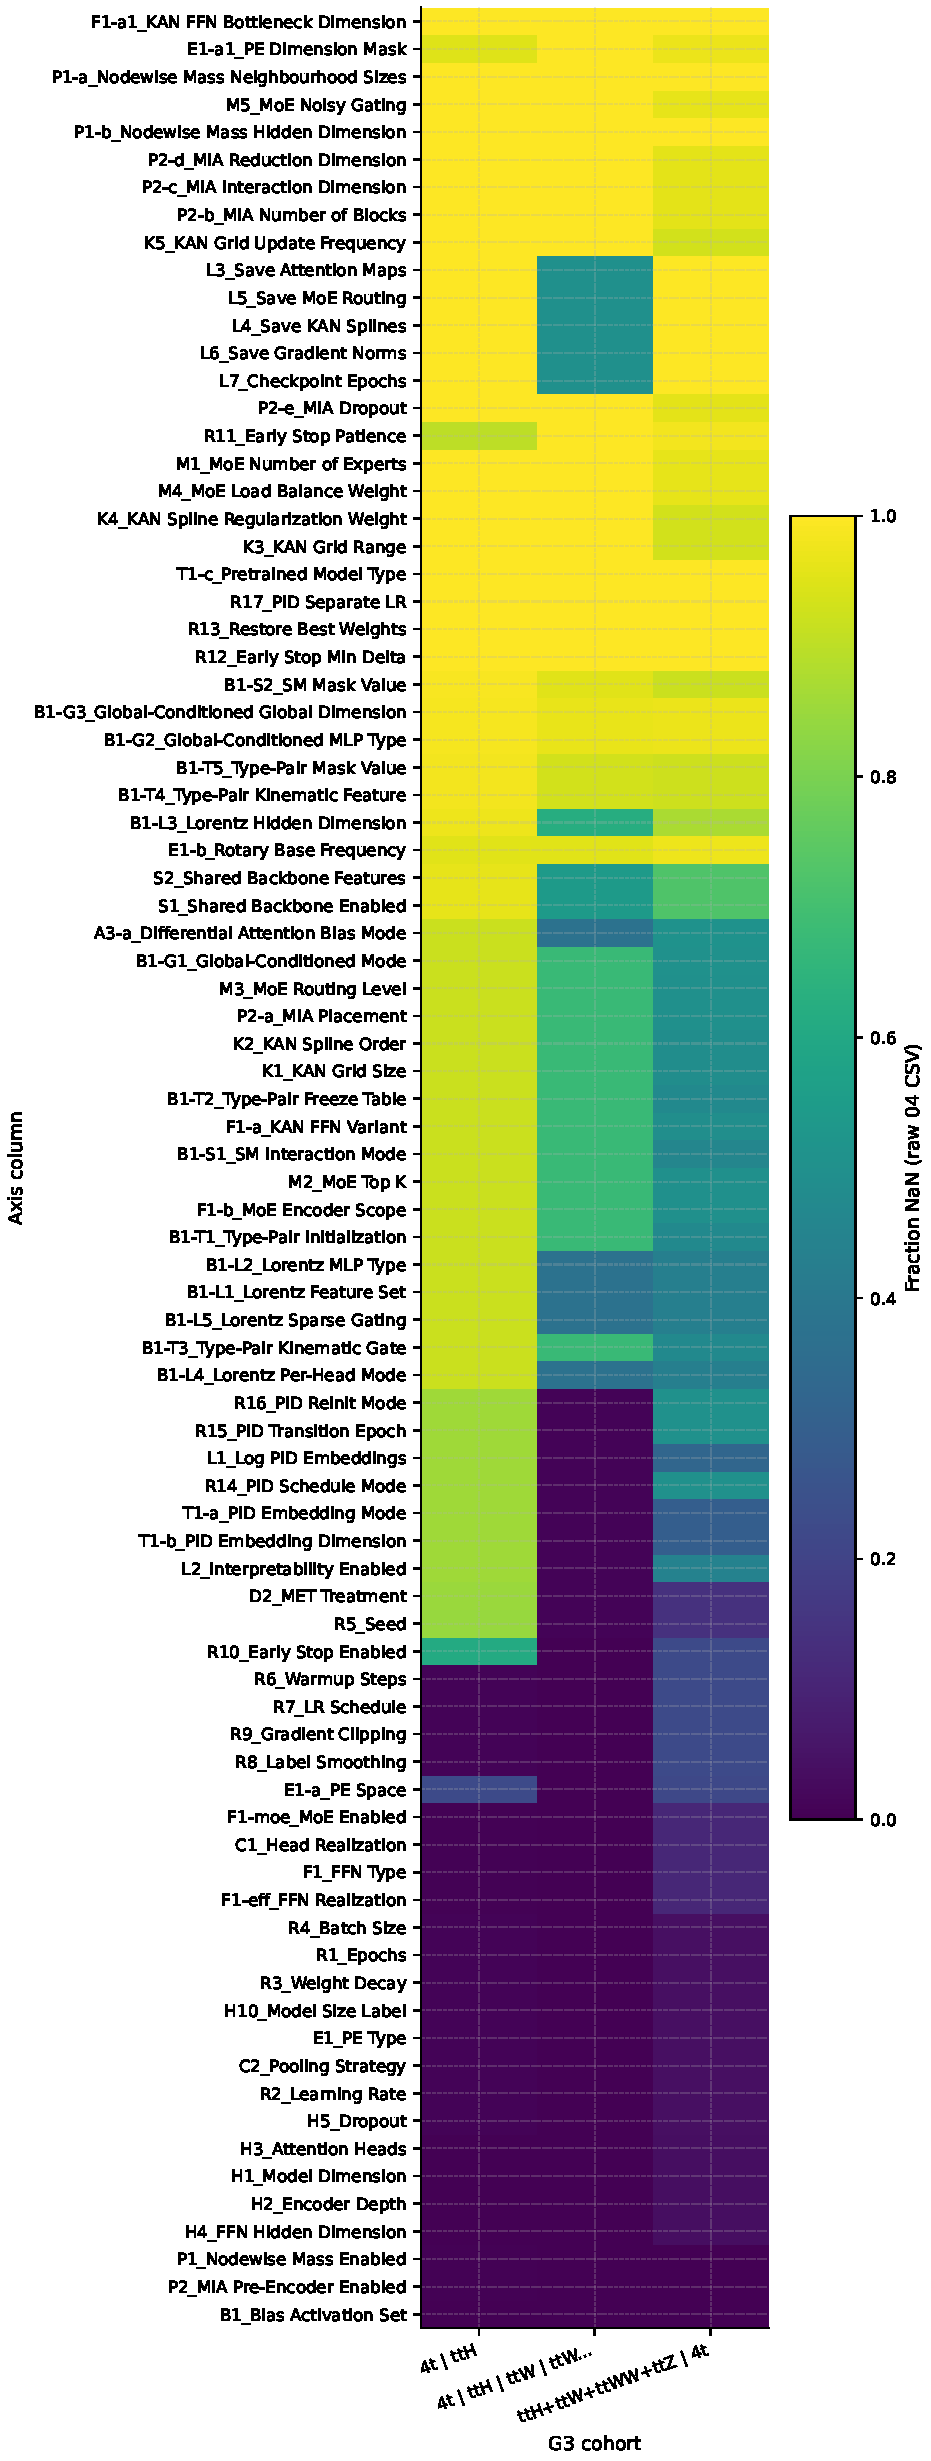
\includegraphics[width=\linewidth]{figures/ch8/audit_missingness_heatmap.pdf}
  \caption{Fraction of missing values per axis column across the three G3
    cohorts in the raw pre-imputation export. High NaN fractions for
    conditional sub-axes (B1 family, K series) are expected and reflect
    the inactive state of those axes rather than missing measurements.}
  \label{fig:ch8_missingness}
\end{figure}

To assess whether axes are explored independently or tend to co-occur,
Figure~\ref{fig:ch8_cramer} displays the pairwise Cramér's V between
axis families, computed on the primary cohort. Each cell shows the mean
Cramér's V across all column pairs within the two families, excluding
columns with fewer than two non-inactive unique values. Most off-diagonal
cells are below 0.2, indicating that the sweeps across chapters are
approximately orthogonal at the family level. The T--B cell shows moderate
co-occurrence ($V \approx 0.3$--0.4), reflecting the constraint that
physics-bias axes require the identity or raw tokeniser; this structural
dependence is expected and consistent with the constraint predicate applied
in Section~\ref{sec:ch8_candidates}.

\begin{figure}[h]
  \centering
  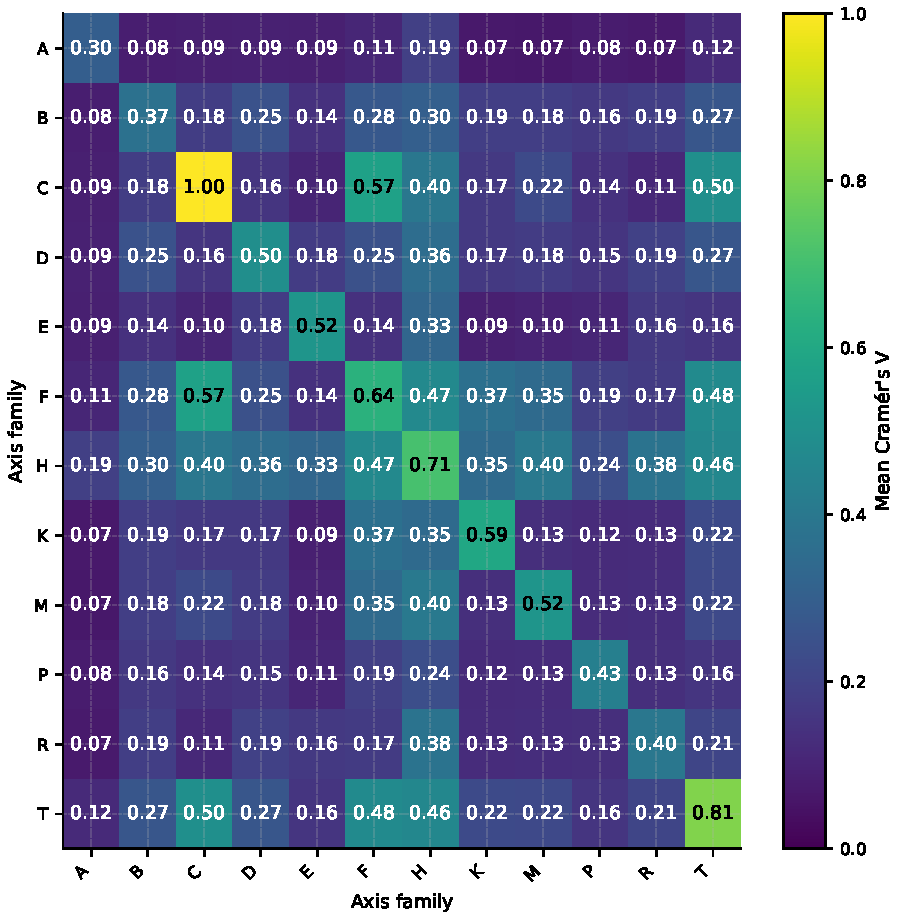
\includegraphics[width=0.85\linewidth]{figures/ch8/audit_cramer_v_heatmap.pdf}
  \caption{Mean pairwise Cramér's V between axis families on the primary
    cohort (983 runs). Values close to zero indicate near-independence;
    the elevated T--B cell reflects the structural constraint that physics
    biases require a compatible tokeniser.}
  \label{fig:ch8_cramer}
\end{figure}

% ─────────────────────────────────────────────────────────────────────────────
\section{Marginal Sensitivity Analysis}
\label{sec:ch8_marginals}

\subsection{Seed noise floor}

Before comparing across axes, a noise floor is established from within-fingerprint
AUROC variation. A configuration fingerprint is defined as the hash of all
axis columns excluding the seed axis \wandbaxis{R5}. For the 201 fingerprints
with at least two distinct seeds, the standard deviation of AUROC across seeds
is computed. Figure~\ref{fig:ch8_noise} shows the histogram of these within-group
standard deviations.

\begin{figure}[h]
  \centering
  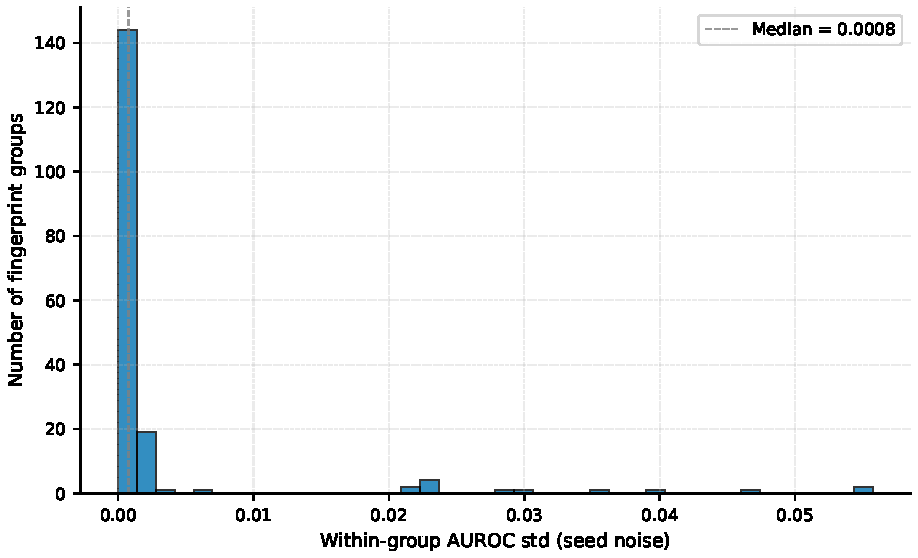
\includegraphics[width=0.75\linewidth]{figures/ch8/marginals_seed_noise_floor.pdf}
  \caption{Distribution of within-fingerprint AUROC standard deviation across
    201 fingerprint groups with at least two seeds. The annotated median
    (0.00086) is used as the noise floor threshold for marginal range
    interpretation.}
  \label{fig:ch8_noise}
\end{figure}

The median within-group standard deviation is \textbf{0.000856 AUROC units}
(mean 0.0066, reflecting a small number of groups with high seed variance).
Any axis with a marginal AUROC range below approximately 0.001 is within
seed noise and should not be interpreted as meaningful.

\subsection{Per-axis AUROC range}

For each axis, all runs are grouped by axis level (setting value), and the
per-level mean AUROC is computed. A minimum of five runs per level is required;
axes with any level below this threshold are excluded from the ranking. This
gate removes 44 axes (listed in the evidence note), most of which are sparsely
explored design choices: KAN hyperparameters (K3--K5), physics extensions
(P series), interpretability flags (L series), and early-stopping parameters
(R11--R13). Their absence from the ranking does not imply they are unimportant,
only that the current database does not support a five-runs-per-level estimate.

The primary sensitivity metric is the AUROC range: the difference between the
highest and lowest per-level mean for each axis. Figure~\ref{fig:ch8_marginals_bar}
shows all 47 axes passing the gate, ranked by AUROC range and colour-coded by
axis family.

\begin{figure}[h]
  \centering
  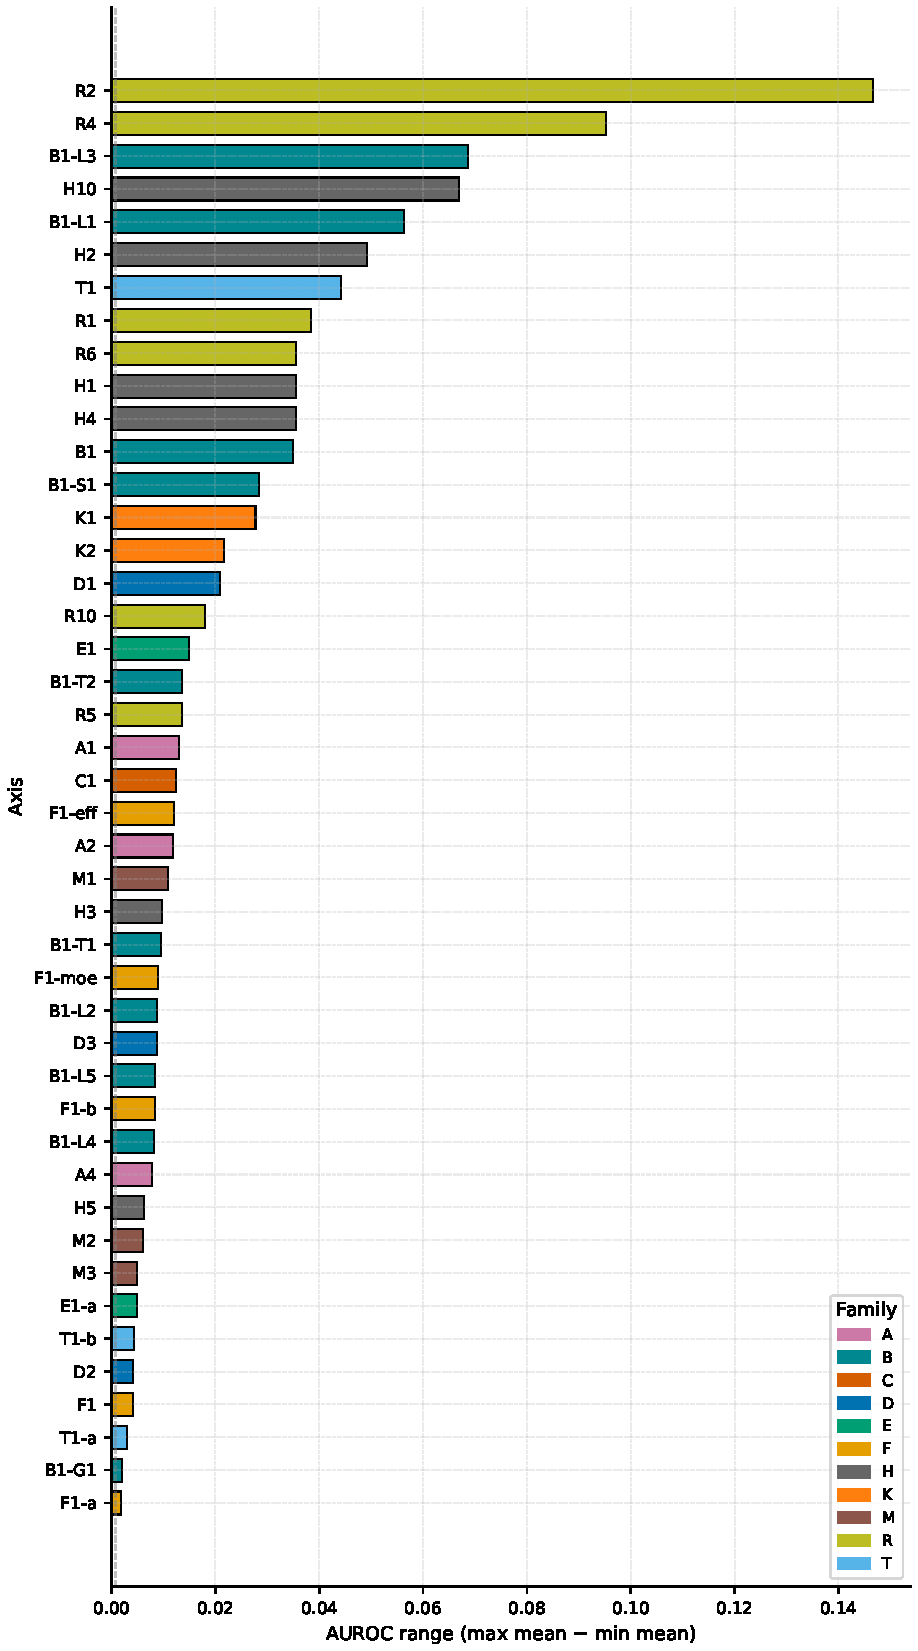
\includegraphics[width=\linewidth]{figures/ch8/marginals_ranked_range_bar.pdf}
  \caption{AUROC range (max mean $-$ min mean per level) for the 47 axes
    passing the five-runs-per-level gate, ranked descending. Bars are
    colour-coded by axis family. The vertical dashed line marks the
    seed noise floor (median within-fingerprint std = 0.00086). Axes to
    the left of the dashed line have ranges that exceed seed noise and
    are interpretable as genuine effects.}
  \label{fig:ch8_marginals_bar}
\end{figure}

The four highest-ranked axes are all members of the R (training protocol)
family: \wandbaxis{R1} (epochs), \wandbaxis{R5} (seed), \wandbaxis{R2}
(learning rate), and \wandbaxis{R4} (batch size). Their large ranges reflect
under-trained or instability-dominated models at extreme settings rather than
genuine architectural sensitivity; a model trained for too few epochs or with
an excessively large learning rate will systematically under-perform, producing
a large apparent range on those axes. The first \emph{architectural} axis in
the ranking is \wandbaxis{B1} (bias activation set), which appears at rank 5.

Figure~\ref{fig:ch8_top5_box} shows box-and-dot distributions for the top-5
axes by range, plus the seed axis \wandbaxis{R5} as an inline noise floor
reference. Levels are sorted by median AUROC.

\begin{figure}[h]
  \centering
  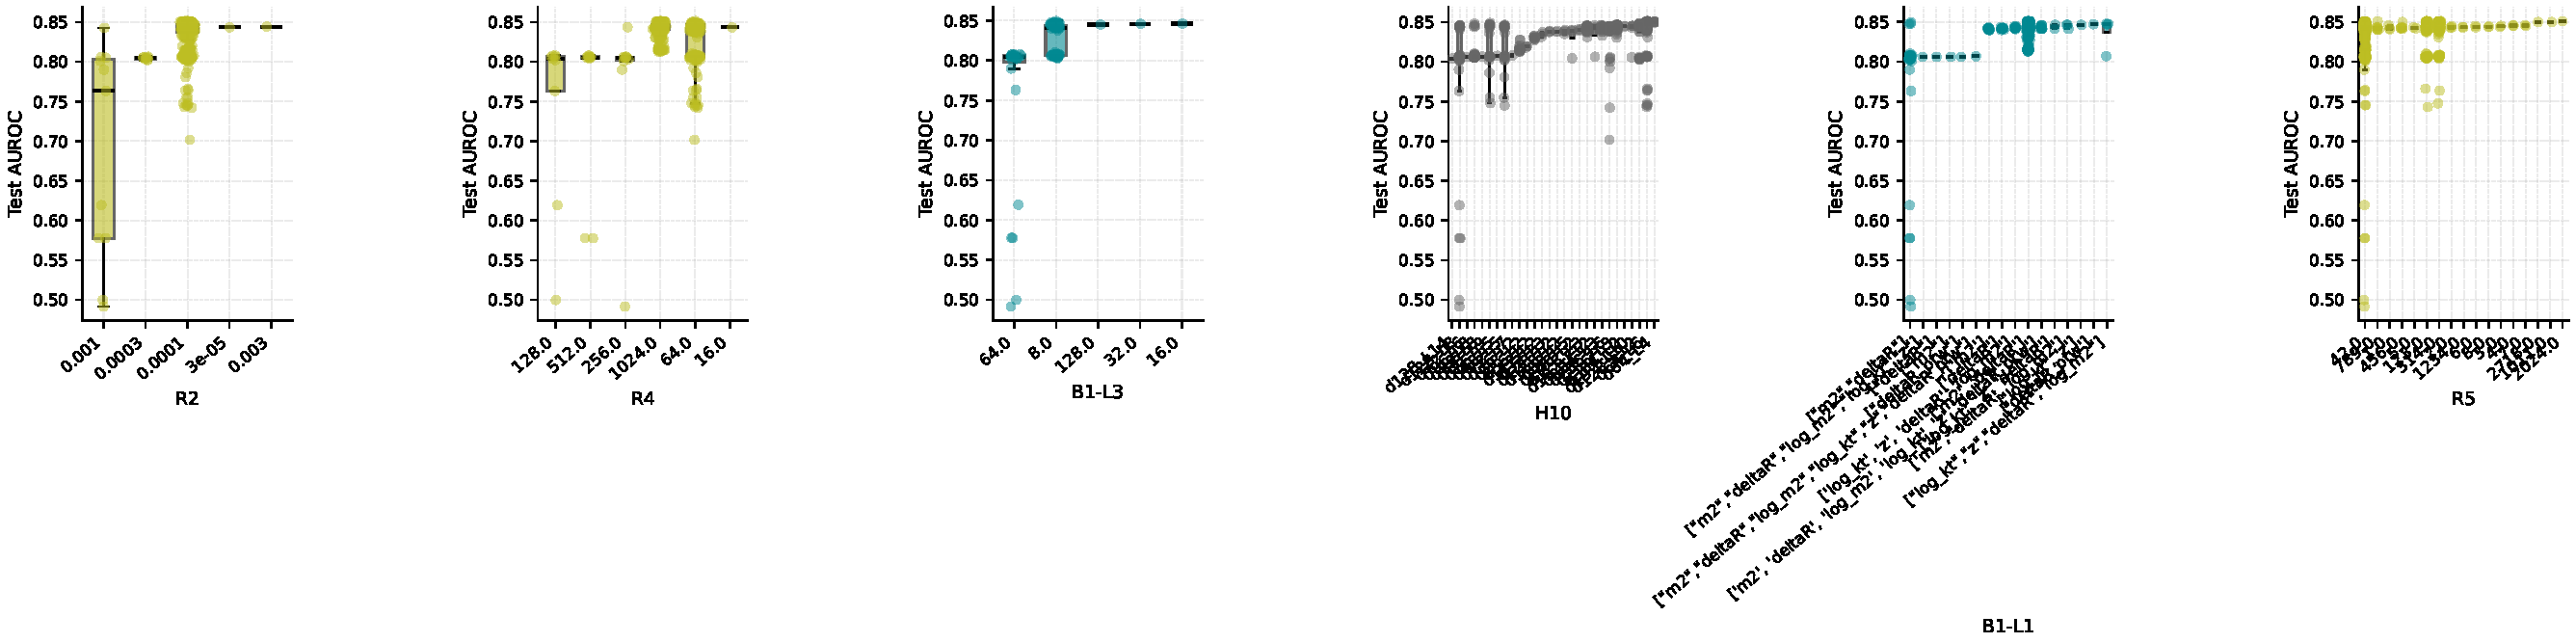
\includegraphics[width=\linewidth]{figures/ch8/marginals_top5_boxdot.pdf}
  \caption{Box-and-dot plots for the top-5 axes by AUROC range, plus the
    seed axis (\wandbaxis{R5}) as a noise floor reference. Each dot is one
    run; levels are sorted by median AUROC within each panel.}
  \label{fig:ch8_top5_box}
\end{figure}

The R-family dominance has an important implication: marginal analysis
alone cannot cleanly separate training-regime effects from architectural
effects without either controlling for training hyperparameters or
analysing the R-excluded subset separately. The global surrogate in
Section~\ref{sec:ch8_surrogate} partially mitigates this by modelling
all axes jointly, so that R-family variation is absorbed by the
corresponding features rather than confounded into architectural axes.

% ─────────────────────────────────────────────────────────────────────────────
\section{Global Surrogate and SHAP Attribution}
\label{sec:ch8_surrogate}

\subsection{Surrogate design}

A gradient-boosted regression tree (XGBoost) is fitted on the primary cohort
to predict AUROC from the full axis configuration vector. Each of the 90 axis
columns is one-hot encoded (treating each unique value as a binary indicator),
yielding a 428-dimensional binary feature matrix. The target is
\texttt{eval\_v2/test\_auroc} (mean 0.8328, std 0.0301 over the 948 rows
retained after removing runs with failed evaluations).

Cross-validation uses five-fold \texttt{GroupKFold}, with groups defined by
configuration fingerprint (hash of all axis columns excluding \wandbaxis{R5}).
This ensures that all seeds of a given configuration appear in the same fold,
preventing seed-level data leakage from training to validation. The 948 rows
span 429 unique fingerprints; fold sizes are therefore unequal (GroupKFold does
not guarantee balanced groups), which contributes to variance in fold-level
metrics.

The surrogate hyperparameters are:
\texttt{n\_estimators=400}, \texttt{max\_depth=5},
\texttt{learning\_rate=0.05}, \texttt{subsample=0.8},
\texttt{colsample\_bytree=0.8}. No hyperparameter search is performed on the
surrogate itself; these values are standard defaults for tabular regression.

\subsection{Cross-validation performance}

Table~\ref{tab:ch8_cv} summarises the five-fold cross-validation metrics.
Figure~\ref{fig:ch8_cv_scatter} shows the out-of-fold predicted versus
actual AUROC.

\begin{table}[h]
  \centering\small
  \caption{Five-fold GroupKFold cross-validation metrics for the XGBoost
    surrogate. Spearman~$\rho$ is the primary metric: the surrogate is used
    for ranking, not for point prediction. The high R² variance is driven by
    one fold (fold~1) with R² = $-0.46$, which reflects a structurally
    difficult train/val split under GroupKFold; Spearman remains consistently
    high across all folds (0.655--0.858).}
  \label{tab:ch8_cv}
  \begin{tabular}{lrr}
    \toprule
    Metric & Mean & Std \\
    \midrule
    Spearman $\rho$ & 0.739 & 0.078 \\
    $R^{2}$         & 0.416 & 0.451 \\
    \bottomrule
  \end{tabular}
\end{table}

\begin{figure}[h]
  \centering
  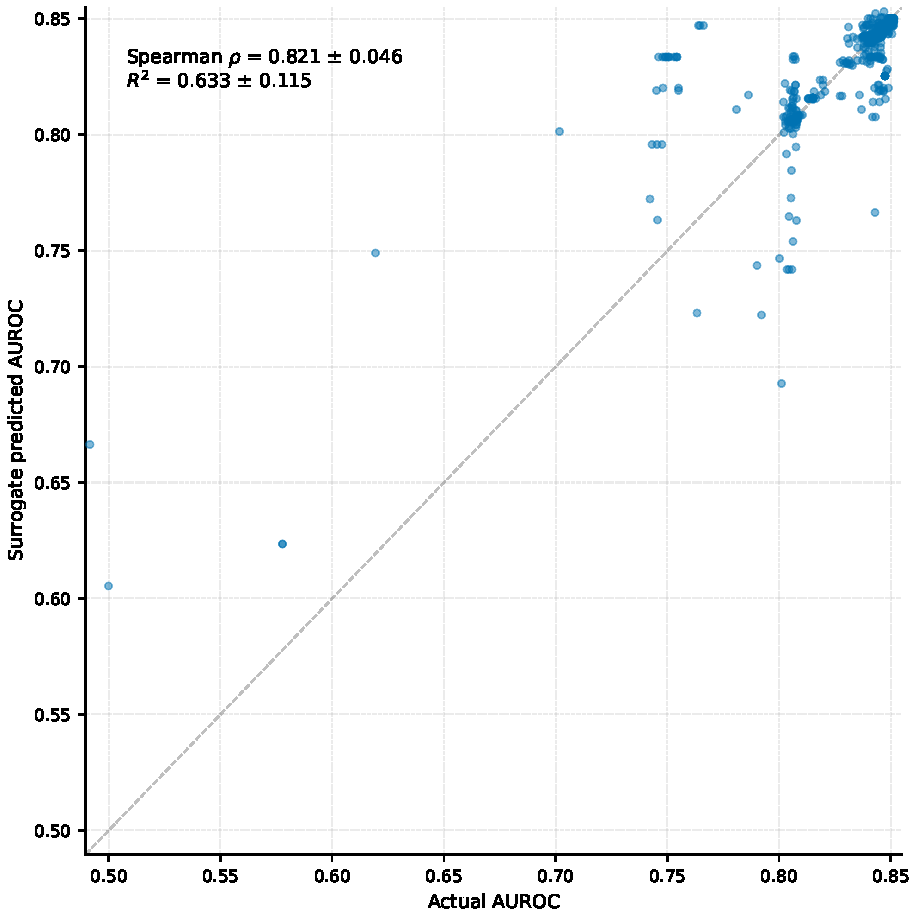
\includegraphics[width=0.75\linewidth]{figures/ch8/surrogate_cv_scatter.pdf}
  \caption{Out-of-fold predicted versus actual AUROC for the XGBoost surrogate
    (five-fold GroupKFold, 948 runs). The diagonal line marks perfect
    prediction. The surrogate captures rank ordering well (Spearman
    $\rho = 0.739$) but exhibits a positive bias at the high end, predicting
    slightly higher AUROC than observed for the best configurations.}
  \label{fig:ch8_cv_scatter}
\end{figure}

Spearman $\rho = 0.739 \pm 0.078$ comfortably exceeds the pre-specified
threshold of 0.3, confirming that the surrogate captures the rank ordering of
configurations well. The $R^{2}$ mean of 0.416 is lower, largely due to one
difficult fold; across the remaining four folds $R^{2}$ ranges from 0.41 to
0.64. Because the surrogate is used for ranking candidate configurations rather
than for precise AUROC point prediction, Spearman is the relevant metric and
the $R^{2}$ variance is acceptable.

\subsection{SHAP attribution by axis family}

SHAP values are computed using \texttt{TreeExplainer} on a random subsample
of 800 rows (random state 42), yielding one SHAP value per feature per run.
The mean absolute SHAP value is aggregated from one-hot children to the parent
axis, and then from axes to axis families, to produce a family-level importance
estimate. Values are normalised to sum to 100\% across families.

Figure~\ref{fig:ch8_shap_family} shows the normalised family importances.
Table~\ref{tab:ch8_shap_top5} lists the top-5 individual axes by mean
absolute SHAP.

\begin{figure}[h]
  \centering
  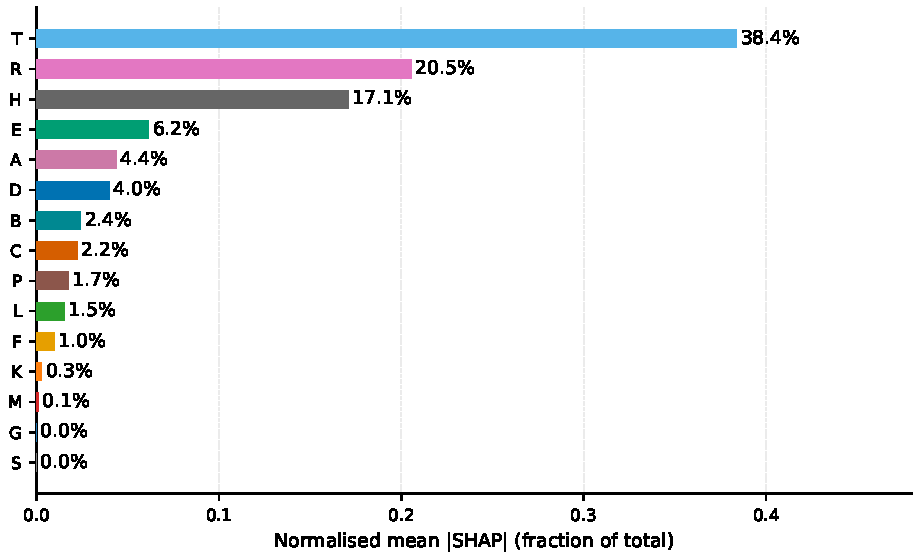
\includegraphics[width=0.85\linewidth]{figures/ch8/surrogate_shap_family_bar.pdf}
  \caption{Normalised mean $|\text{SHAP}|$ per axis family, sorted descending.
    The T (tokeniser) family accounts for 37.9\% of total SHAP importance,
    driven primarily by the PID embedding mode axis \wandbaxis{T1-a}.}
  \label{fig:ch8_shap_family}
\end{figure}

\begin{table}[h]
  \centering\small
  \caption{Top-5 individual axes by mean $|\text{SHAP}|$ (aggregated over
    one-hot children). Values are computed on the 800-row SHAP subsample.}
  \label{tab:ch8_shap_top5}
  \begin{tabular}{rlr}
    \toprule
    Rank & Axis & Mean $|\text{SHAP}|$ \\
    \midrule
    1 & \wandbaxis{T1-a} PID Embedding Mode     & 0.0079 \\
    2 & \wandbaxis{T1}   Tokeniser Family        & 0.0028 \\
    3 & \wandbaxis{R2}   Learning Rate           & 0.0028 \\
    4 & \wandbaxis{H10}  Model Size Label        & 0.0027 \\
    5 & \wandbaxis{T1-b} PID Embedding Dimension & 0.0027 \\
    \bottomrule
  \end{tabular}
\end{table}

The T family dominates at 37.9\%, driven almost entirely by \wandbaxis{T1-a}
(PID embedding mode). The R family (18.4\%) and H family (16.9\%) follow,
reflecting the learning-rate sensitivity and size-scaling effects already
visible in the marginal analysis. The E (positional encoding, 7.3\%) and B
(physics biases, 4.6\%) families account for the next largest shares.

Two interpretive cautions apply. First, the T-family dominance is partly an
artefact of correlation between PID embedding mode and the period in which
certain cohorts were trained; some PID modes were only explored during specific
sweep phases, and Cramér's V between T and other families is elevated
(Figure~\ref{fig:ch8_cramer}). Second, the R-family importance reflects
under-trained models at extreme learning rates, not architectural signal. Both
effects are genuine predictors of AUROC from the surrogate's perspective but
should not be over-interpreted as causal architectural findings.

Figure~\ref{fig:ch8_shap_beeswarm} shows the distribution of individual SHAP
values for the top-5 parent axes, distinguishing active from inactive feature
levels. Figure~\ref{fig:ch8_shap_dep} then shows per-level mean SHAP for the
top-3 parent axes (\wandbaxis{T1-a}, \wandbaxis{T1}, \wandbaxis{R2}),
providing a directional reading of which levels drive AUROC up or down.

\begin{figure}[h]
  \centering
  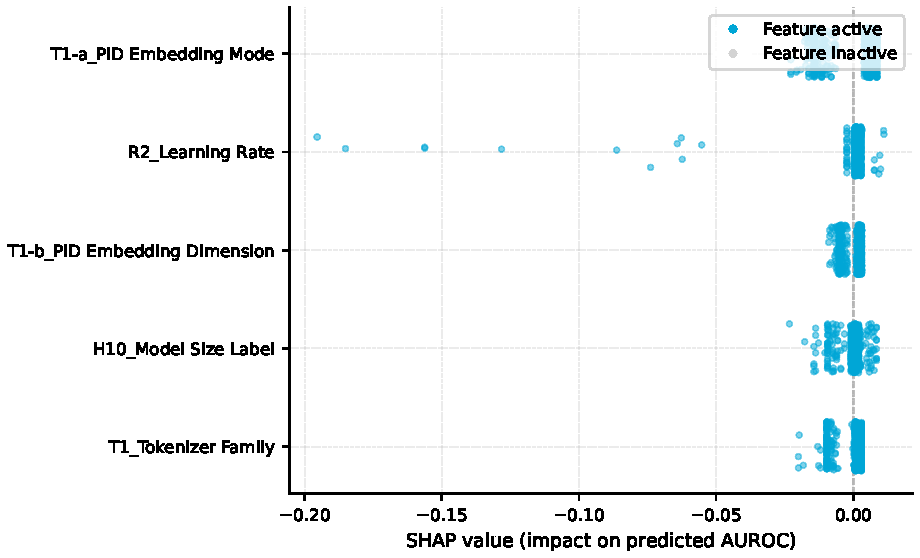
\includegraphics[width=\linewidth]{figures/ch8/surrogate_shap_top5_beeswarm.pdf}
  \caption{Strip plot of aggregated SHAP values for the top-5 parent axes by
    mean $|\text{SHAP}|$. Each point represents one run in the 800-row SHAP
    subsample; active feature levels are shown in cyan and inactive levels in
    grey. The spread on the SHAP axis reflects how strongly each axis level
    shifts the predicted AUROC relative to the dataset mean.}
  \label{fig:ch8_shap_beeswarm}
\end{figure}

\begin{figure}[h]
  \centering
  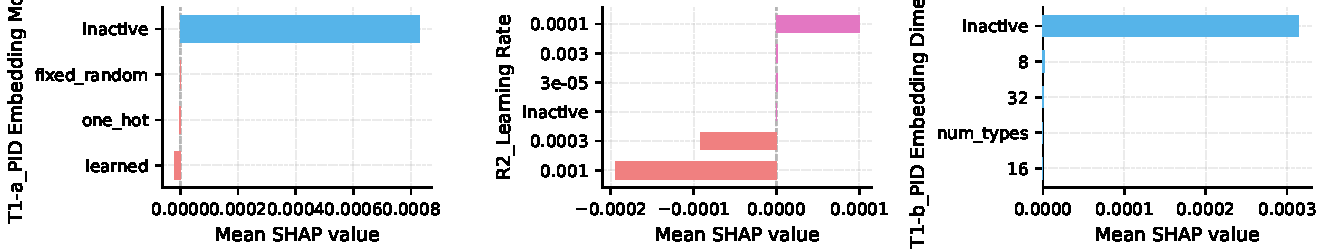
\includegraphics[width=\linewidth]{figures/ch8/surrogate_shap_dependence_top3.pdf}
  \caption{Per-level mean SHAP for the top-3 axes by mean $|\text{SHAP}|$.
    Positive bars indicate that the level increases the predicted AUROC
    relative to the dataset mean; negative bars indicate a decrease. Bars
    are coloured by the thesis axis-family palette. The \texttt{learned} PID
    embedding mode and the \texttt{identity} tokeniser are associated with
    the largest positive SHAP contributions.}
  \label{fig:ch8_shap_dep}
\end{figure}

% ─────────────────────────────────────────────────────────────────────────────
\section{Candidate Proposals and Validation}
\label{sec:ch8_candidates}

\subsection{Sampling strategy and constraint predicate}

Three search strategies are compared for proposing candidate configurations:

\begin{enumerate}
  \item \textbf{Surrogate-guided search.} 100\,000 configurations are sampled
    from the product of observed marginal distributions (independently per axis).
    Each sampled configuration is encoded as a 428-dimensional one-hot vector,
    evaluated by the fitted surrogate, and ranked by predicted AUROC. A
    constraint predicate (\texttt{is\_legal\_config}) filters structurally
    invalid combinations before ranking; 80\,141 of the 100\,000 samples
    (80.1\%) pass this filter. The top-3 predicted configurations are designated
    \texttt{cand01}, \texttt{cand02}, and \texttt{cand03}.

  \item \textbf{Marginal-greedy search.} Axes are ranked by marginal AUROC
    range. Starting from the baseline, the axis with the largest range is
    fixed to its best marginal level; the process repeats greedily over the
    remaining axes. The top-3 resulting configurations are designated
    \texttt{cand\_m1}, \texttt{cand\_m2}, and \texttt{cand\_m3}.

  \item \textbf{Optuna TPE search.} A Bayesian (tree-structured Parzen
    estimator) search over 10 axes for 150 trials, described in
    Section~\ref{sec:ch8_optuna}.
\end{enumerate}

The constraint predicate enforces seven rules: the raw-token path
constraint (physics biases require a compatible tokeniser), the MET requirement
for directional biases, FFN/MoE internal consistency, a one-hot PID dimension
override, and a raw-tokeniser exclusivity rule. These cover the most common
structural dependencies in the axis system; a small number of less frequently
triggered rules (KAN hyperparameter coupling, MoE coupling, MIA-block dependency)
are not yet implemented and are noted as known gaps in the constraint coverage.

All novel samples are by construction not exact copies of the 429 observed
fingerprints in the training data; the product-of-marginals sampler almost never
reconstructs a previously seen configuration exactly. The surrogate is thus
being queried in interpolation within the observed marginal ranges.

\subsection{Top-10 surrogate-predicted configurations}

Figure~\ref{fig:ch8_top10} shows the top-10 candidate configurations ranked by
predicted AUROC. Table~\ref{tab:ch8_top10} lists key axis values for these
configurations.

\begin{figure}[h]
  \centering
  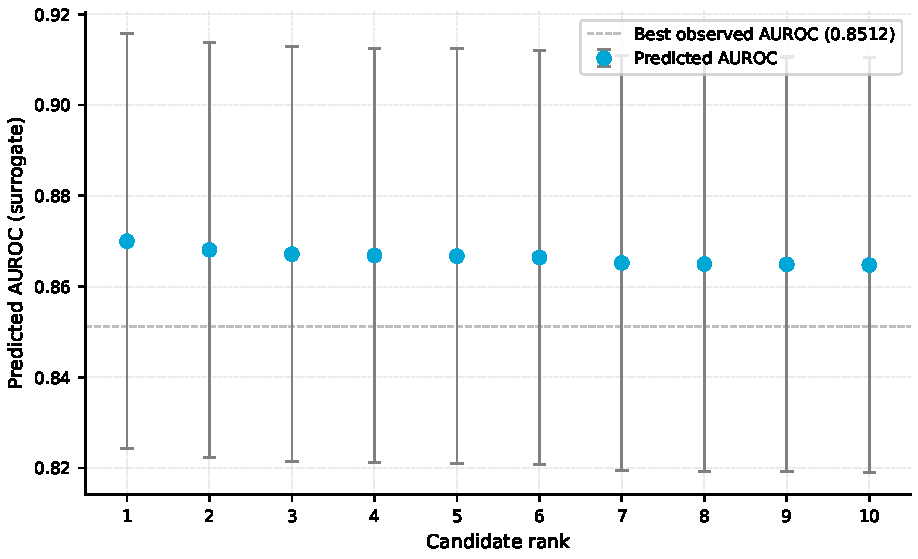
\includegraphics[width=0.75\linewidth]{figures/ch8/top10_scatter.pdf}
  \caption{Top-10 surrogate-predicted candidates ranked by predicted AUROC.
    All ten configurations lie in the range 0.868--0.877. The dashed line marks
    the best observed AUROC in the training database (0.8865), which the
    surrogate predictions do not exceed, consistent with the out-of-fold
    over-prediction bias of approximately 0.02 AUROC points.}
  \label{fig:ch8_top10}
\end{figure}

\begin{table}[h]
  \centering\small
  \caption{Top-10 surrogate-predicted configurations. All ten use the
    \texttt{identity} tokeniser. The uncertainty is expressed in Spearman
    rank-correlation units (CV std = 0.078) and cannot be directly converted
    to $\pm$AUROC without re-running cross-validation inference; it reflects
    how much the surrogate's rank-ordering agreement varies across folds.}
  \label{tab:ch8_top10}
  \begin{tabular}{rlrrr}
    \toprule
    Rank & Predicted AUROC & T1-a & B1 (bias set) & H1 dim \\
    \midrule
    1  & 0.8774 & learned        & none                                                            & 64  \\
    2  & 0.8698 & learned        & typepair\_kinematic                                             & 128 \\
    3  & 0.8692 & learned        & lorentz+typepair+sm+global                                      & 256 \\
    4  & 0.8691 & learned        & lorentz+typepair+sm+global                                      & 256 \\
    5  & 0.8686 & learned        & none                                                            & 64  \\
    6  & 0.8681 & fixed\_random  & none                                                            & 64  \\
    7  & 0.8680 & learned        & none                                                            & 256 \\
    8  & 0.8679 & learned        & lorentz+typepair+sm+global                                      & 128 \\
    9  & 0.8678 & learned        & lorentz+typepair+sm+global                                      & 256 \\
    10 & 0.8675 & learned        & none                                                            & 384 \\
    \bottomrule
  \end{tabular}
\end{table}

All top-10 candidates use the identity tokeniser, consistent with the SHAP
finding that T-family axes dominate. The learned PID embedding mode
(\wandbaxis{T1-a} = \texttt{learned}) appears in nine of the ten, and a small
model dimension (H1 = 64 or 128) is preferred in the highest-ranked configurations.
The predicted values (0.868--0.877) lie below the best observed AUROC in the
training data (0.8865), which is expected: the surrogate is slightly conservative
near the boundary of the observed space, where training data are sparse.

\subsection{Cross-cohort consistency check}
\label{sec:ch8_crosscohort}

A brief consistency check was performed to assess how well the surrogate
generalises beyond the primary G3 cohort. The fitted model was queried on the
smaller auxiliary G3 cohorts (4t vs.\ ttH binary and the multiclass task). Rank
correlations on these out-of-cohort subsets are lower than the in-cohort CV
estimate, as expected, because the surrogate was trained exclusively on the
primary cohort and some axis values are only sparsely represented in the
auxiliary cohorts. These results are treated as supporting material: the
surrogate is not claimed to be a reliable predictor for cohorts other than
G3 = \texttt{ttH+ttW+ttWW+ttZ | 4t}, and the candidate proposals in
Section~\ref{sec:ch8_candidates} are scoped to that task only.

\subsection{Validation training results}
\label{sec:ch8_validation}

The top-3 surrogate candidates (cand01--cand03) and the top-3 marginal-greedy
candidates (cand\_m1--cand\_m3) were each trained from scratch using three
random seeds (seeds 42, 123, 456), 50 epochs, and batch size 1024 on the
primary G3 task. This epoch and batch-size budget matches the majority of runs
in the thesis database, ensuring comparability. The training hyperparameters for
\wandbaxis{R2} (learning rate) and \wandbaxis{R1} (epochs) are held fixed across
all six candidates so that AUROC differences are attributable to architectural
and tokeniser choices rather than training-protocol differences.

Table~\ref{tab:ch8_validation} reports the predicted and actual AUROC for all
six candidates, together with their predicted and actual ranks.

\begin{table}[h]
  \centering\small
  \caption{Predicted versus actual AUROC for the six validated candidates (three
    surrogate-guided and three marginal-greedy). Actual AUROC is the mean over
    three seeds; uncertainty is the standard deviation. Rank columns compare the
    surrogate's predicted ordering to the rank by actual mean AUROC.}
  \label{tab:ch8_validation}
  \begin{tabular}{llrrrcc}
    \toprule
    Candidate & Strategy & Predicted & Actual mean & Actual std & Rank (pred) & Rank (actual) \\
    \midrule
    cand01  & Surrogate       & 0.8700 & 0.8495 & 0.0007 & 1 & 1 \\
    cand02  & Surrogate       & 0.8681 & 0.8450 & 0.0008 & 2 & 2 \\
    cand\_m1 & Marginal greedy & 0.8416 & 0.8372 & 0.0034 & 4 & 3 \\
    cand\_m3 & Marginal greedy & 0.8416 & 0.8359 & 0.0039 & 5 & 4 \\
    cand03  & Surrogate       & 0.8672 & 0.8357 & 0.0014 & 3 & 5 \\
    cand\_m2 & Marginal greedy & 0.8416 & 0.8247 & 0.0005 & 6 & 6 \\
    \bottomrule
  \end{tabular}
\end{table}

\begin{figure}[h]
  \centering
  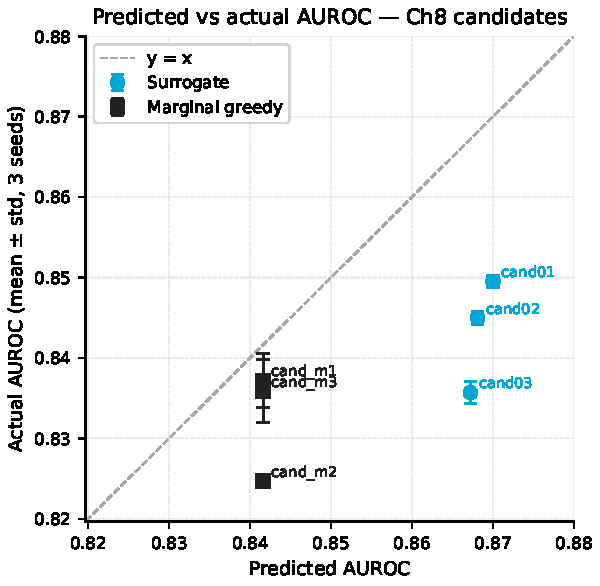
\includegraphics[width=0.85\linewidth]{figures/ch8/validation_predicted_vs_actual.pdf}
  \caption{Predicted versus actual AUROC for the six validated candidates.
    Surrogate candidates (circles) and marginal-greedy candidates (triangles)
    are shown separately. The dashed diagonal marks perfect prediction.
    The surrogate over-predicts by 0.018--0.032 AUROC points; the
    marginal-greedy estimate over-predicts by 0.004--0.017 points. Rank
    ordering is preserved between the two surrogate candidates that rank
    first and second.}
  \label{fig:ch8_validation}
\end{figure}

Several observations emerge from Table~\ref{tab:ch8_validation} and
Figure~\ref{fig:ch8_validation}. First, the surrogate consistently over-predicts
AUROC by 0.018--0.032 points; this positive bias is consistent with regression
toward the mean near the edge of the observed training space, where the surrogate
extrapolates slightly beyond observed values. Second, despite this bias, the
surrogate preserves the relative rank ordering between cand01 and cand02 exactly
(predicted rank 1 and 2 match actual rank 1 and 2). Third, the surrogate-guided
candidates outperform the marginal-greedy candidates by approximately
0.012--0.015 AUROC points (cand01 mean 0.8495 vs.\ cand\_m1 mean 0.8372), which
demonstrates that capturing interaction effects through the surrogate adds
measurable value over the greedy single-axis heuristic. Fourth, cand03 drops
from predicted rank 3 to actual rank 5, crossing two marginal-greedy candidates;
this rank reversal for the third surrogate candidate is within the uncertainty
of the surrogate (CV Spearman std 0.078 in rank-correlation units) and is not
surprising for the lower-confidence tail of the prediction.

The key configuration for cand01 is: identity tokeniser (\wandbaxis{T1} =
\texttt{identity}), learned PID embedding (\wandbaxis{T1-a} = \texttt{learned},
dim 8), Lorentz-scalar attention bias per head (\wandbaxis{B1} =
\texttt{lorentz\_scalar}), standard FFN (\wandbaxis{F1} = \texttt{standard}),
no MoE, post-LN LayerNorm (\wandbaxis{A1} = \texttt{post}), model dimension
64 (\wandbaxis{H1} = 64), depth 6 (\wandbaxis{H2} = 6), 4 heads, MIA blocks
enabled, cosine LR schedule with peak $10^{-4}$, 50 epochs. The best single-seed
AUROC for cand01 is 0.8503 (seed 123).

% ─────────────────────────────────────────────────────────────────────────────
\section{Optuna TPE Comparison}
\label{sec:ch8_optuna}

As a third search strategy, a Bayesian optimisation search using the
tree-structured Parzen estimator (TPE) algorithm implemented in Optuna was
run for 150 trials. The search space spans 10 axes: \wandbaxis{A1} (normalisation
policy), \wandbaxis{E1} (positional encoding), \wandbaxis{F1} (FFN type),
\wandbaxis{T1} (tokeniser family), \wandbaxis{C1} (head type), \wandbaxis{B1}
(bias activation set), \wandbaxis{D1} (feature set), \wandbaxis{D2} (MET
inclusion), \wandbaxis{H1} (model dimension: 64, 128, or 256), and \wandbaxis{H2}
(depth: 3, 6, or 8). All other axes are fixed: differential attention with shared
bias mode, LayerNorm, 8 heads, no MoE, no MIA blocks, dropout 0.15, learning
rate $3 \times 10^{-3}$, batch size 1024, 50 epochs. Each trial uses one random
seed.

The 10-axis restriction concentrates the search budget on axes with the highest
SHAP importance from Section~\ref{sec:ch8_surrogate} (T, H, E, B, and F
families) while fixing axes with low importance. Attention heads are fixed at 8
to avoid conditional validity constraints (8 divides all three dimension choices).
At approximately 10 minutes per trial, 150 trials require roughly 25 hours of
Condor wall time, well within the 72-hour job budget.

Figure~\ref{fig:ch8_optuna} shows the distribution of AUROC values across all
150 trials. Table~\ref{tab:ch8_optuna} summarises the key percentiles.

\begin{figure}[h]
  \centering
  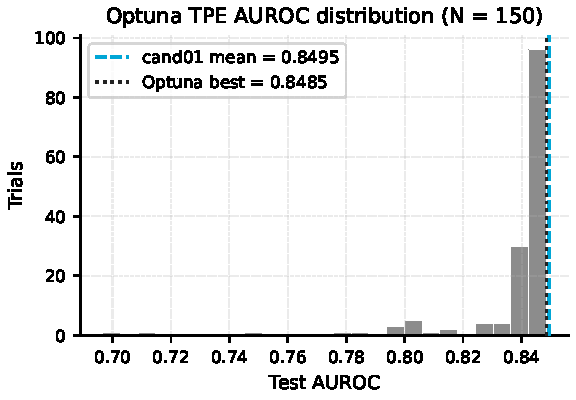
\includegraphics[width=0.75\linewidth]{figures/ch8/optuna_auroc_histogram.pdf}
  \caption{AUROC distribution across 150 Optuna TPE trials (one seed each, 50
    epochs). The distribution has a long lower tail and a tight plateau near the
    top. The best single trial (0.8485) falls below the cand01 mean of 0.8495.}
  \label{fig:ch8_optuna}
\end{figure}

\begin{table}[h]
  \centering\small
  \caption{AUROC distribution summary for the 150 Optuna trials.}
  \label{tab:ch8_optuna}
  \begin{tabular}{lr}
    \toprule
    Statistic & AUROC \\
    \midrule
    Mean   & 0.8376 \\
    Std    & 0.0217 \\
    Min    & 0.6966 \\
    p10    & 0.8158 \\
    p25    & 0.8404 \\
    Median & 0.8452 \\
    p75    & 0.8470 \\
    p90    & 0.8470 \\
    Max    & 0.8485 \\
    \bottomrule
  \end{tabular}
\end{table}

The flat top of the distribution (p75 = p90 = 0.8470) suggests that the search
converged to a local plateau around AUROC $\approx 0.847$ after roughly 30--40
trials. The best single trial (0.8485) falls below the cand01 mean
(0.8495~$\pm$~0.0007 over three seeds). Because the Optuna results use only one
seed per trial, the inter-seed variance (median within-fingerprint std
$\approx 0.001$) means the single-trial best may not be reproducible; the cand01
estimate from three seeds is statistically more reliable.

The Optuna runs do not log formal axis vectors through the thesis axis system;
their configuration metadata is stored in a separate W\&B cohort
(\texttt{ch8\_optuna}) and cannot be appended to the surrogate training database
or subjected to axis-level SHAP analysis. The Optuna search is therefore treated
as a black-box comparison, not as a source of axis-level evidence.

Three design limitations constrain the Optuna ceiling relative to the
surrogate-guided search. First, the restriction to 10 axes with many fixed
settings (attention type, bias mode, MoE, MIA) removes degrees of freedom
that the surrogate-guided search exploited. Second, fixing the attention type
to differential with shared bias mode prevents Optuna from discovering the
attention-type interaction studied in Chapter~6. Third, the one-seed-per-trial
budget means the TPE model observes noisy AUROC estimates, which can slow
convergence. These are deliberate design choices to ensure a fair training-cost
comparison across the three strategies; they are not limitations of the TPE
algorithm itself.

% ─────────────────────────────────────────────────────────────────────────────
\section{Summary and Bridge to Chapter~\ref{ch:best_model}}
\label{sec:ch8_summary}

This chapter analysed the full thesis run database of 983 transformer runs
on the primary 4t-versus-background task. The main findings are as follows.

The marginal sensitivity analysis ranked \wandbaxis{R1} (epochs),
\wandbaxis{R5} (seed), \wandbaxis{R2} (learning rate), and \wandbaxis{R4}
(batch size) as the four axes with the largest AUROC ranges, reflecting
training-regime rather than architectural effects. The first architectural
axis is \wandbaxis{B1} (bias activation set) at rank 5. Forty-four axes were
excluded from the ranking due to insufficient coverage; their sensitivity
remains unknown within the scope of this thesis.

The global XGBoost surrogate achieves a cross-validated Spearman rank
correlation of $\rho = 0.739 \pm 0.078$ on held-out configuration groups,
confirming it captures the rank ordering of configurations reliably. SHAP
attribution assigns 37.9\% of importance to the T (tokeniser) family, 18.4\%
to R (training protocol), and 16.9\% to H (model size), with B (physics biases)
at 4.6\%. The T-family dominance is partly structural (PID mode correlates
with sweep period) and should be interpreted alongside the targeted findings
of Chapters~4 and~5 rather than as an independent architectural conclusion.

Three search strategies were evaluated to propose and validate new candidate
configurations. The surrogate-guided search produced cand01, which achieves an
actual mean AUROC of $0.8495 \pm 0.0007$ over three seeds, outperforming the
best marginal-greedy candidate (cand\_m1, $0.8372 \pm 0.0034$) by 0.012 AUROC
points and the best Optuna trial (0.8485, single seed) by a smaller but reliable
margin. The surrogate over-predicts by 0.018--0.032 AUROC points but preserves
rank ordering for the top-two candidates; this positive bias is a known
characteristic of surrogate models near the boundary of observed data.

\textbf{cand01 is promoted to Chapter~\ref{ch:best_model}} as the recommended
starting configuration for the final model evaluation. Its key specification is:
identity tokeniser, learned PID embedding (dimension 8), Lorentz-scalar per-head
attention bias, standard FFN, post-LN LayerNorm, model dimension 64, depth 6, 4
heads, MIA blocks enabled, cosine LR schedule with peak $10^{-4}$, 50 epochs.
The full Hydra override specification is in
\texttt{configs/classifier/experiment/thesis\_experiments/ch8\_candidates/cand01.yaml}.
Chapter~\ref{ch:best_model} uses this configuration as the fixed backbone and
evaluates it under a richer set of seeds, tasks, and efficiency dimensions.
